\begin{frame}
	\frametitle{Base de dados}
	
	\only<1>{
	\par A principio a base de dados usada será a \textit{Open access database of EEG signals recorded during imagined speech}\cite{10.1117/12.2255697} para testes preliminares e desenvolvimento dos algoritmos de filtragem e analise dos sinais.\newline
	
	\begin{quote}
		Este banco de dados contém as gravações de EEG durante a pronúncia imaginada de vogais e comandos, bem como EEG e gravações de áudio durante a pronúncia de vogais e comandos. A amostra é composta por 15 voluntários argentinos entre 24 e 28 anos de idade, de ambos os sexos; sendo 7 mulheres e 8 homens. O objetivo do banco de dados é permitir a acessibilidade dos registros de EEG durante a fala imaginada para futuras pesquisas voltadas para o desenvolvimento de dispositivos BCI que permitam a classificação de palavras a partir de sua imaginação. 
		\cite{10.1117/12.2255697}
	\end{quote}
	}
	\only<2>{
	\par A base está estruturada de forma que cada linha corresponda a um sujeito sendo que, em cada linha, os dados se organizam do seguinte modo:
	\begin{columns}
		\begin{column}{0.4\textwidth}
			\par F3, F4, C3, C4, P3, P4 são as identificações de cada eletrodo.
			\begin{itemize}
				\item F3 - 0:4095
				\item F4 - 4096:8191
				\item C3 - 8192:12287
				\item C4 - 12288:16383
				\item P3 - 16384:20479
				\item P4 - 20480:24575
				\item modalidade - 24576:24576
				\item estímulo - 24577:24577
			\end{itemize}
			
		\end{column}
		\begin{column}{0.6\textwidth}
			\begin{figure}
				\centering
				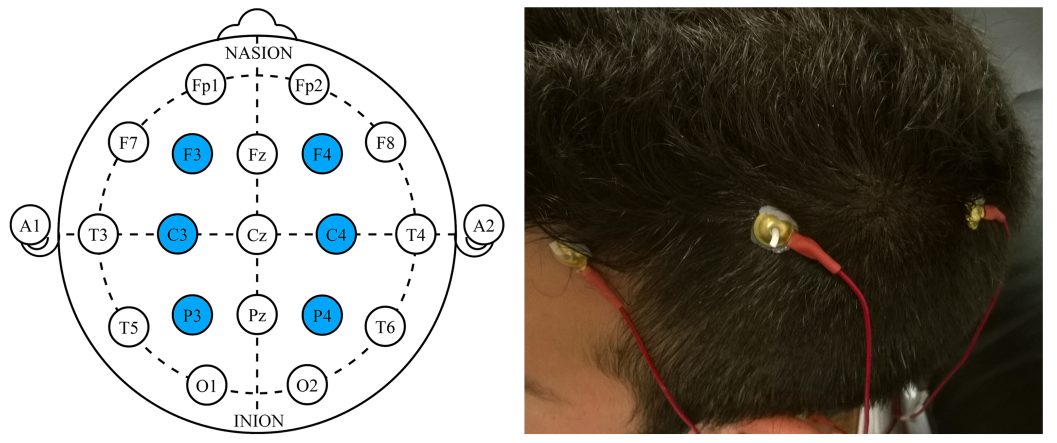
\includegraphics[width=\linewidth]{images/visu03}
				\caption{Colocação dos sensores: Nota-se que apenas uma parcela do sistema 10-20 de colocação dos sensores foi utilizada. Fonte: \cite{10.1117/12.2255697}}
				\label{fig:visu03}
			\end{figure}
			
		\end{column}
	\end{columns}
	}
	\only<3>{
		\par A modalidade pode ser: 1 - Imaginada, 2 - Pronunciada.
		\par O valor do estímulo pode se encaixar em uma das categorias por vez:
		\begin{itemize}
			\item Letras:
			1 - A, 2 - E, 3 - I, 4 - O, 5 - U
			\item Comandos:
			6 - Arriba, 7 - Abajo, 8 - Adelante, 9 - Atrás, 10 - Derecha, 11 - Izquierda	
		\end{itemize}
		
		\par Na pesquisa pretende-se gerar uma base própria em parceria com as instituições de saúde da cidade.	
	}
\end{frame}
\begin{frame}
	\frametitle{Amostra dos dados na base}
	\only<1>{
	\begin{figure}
		\centering
		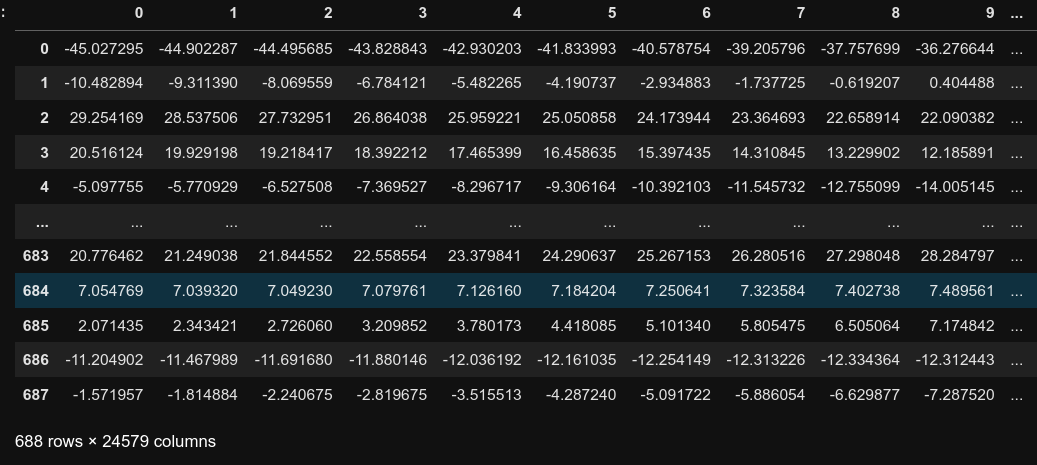
\includegraphics[width=\linewidth]{images/visu04}
		\caption{Primeiras colunas da base de dados}
		\label{fig:visu04}
	\end{figure}
	}
	\only<2>{
	\begin{figure}
		\centering
		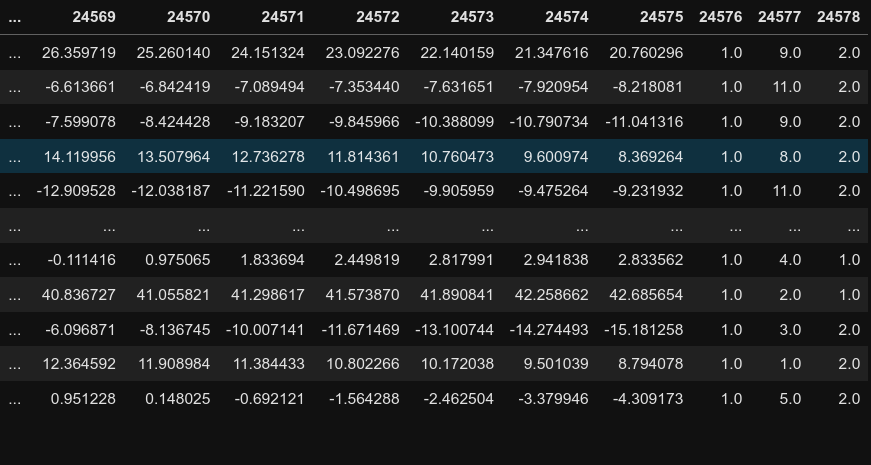
\includegraphics[width=.9\linewidth]{images/visu05}
		\caption{Últimas colunas da base de dados}
		\label{fig:visu05}
	\end{figure}
	}
\end{frame}
\begin{frame}
	\frametitle{Pré-processamento}
	\par Objetivando facilitar a manipulação dos dados foram criados os agrupamentos mostrados na figura \ref{fig:visu06}.
	\begin{figure}
		\centering
		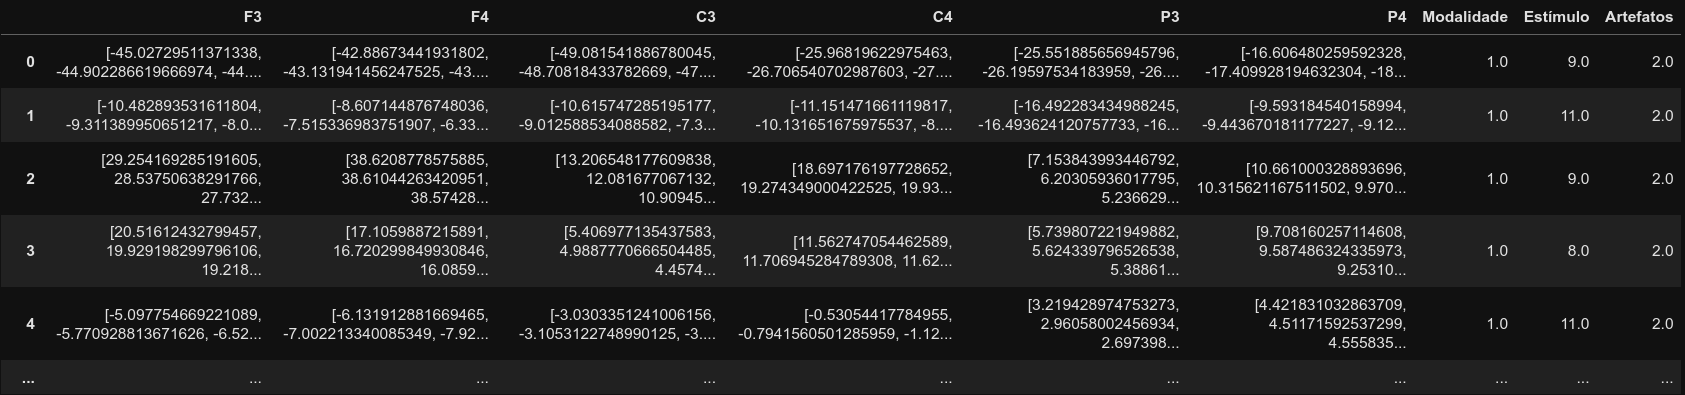
\includegraphics[width=\linewidth]{images/visu06}
		\caption{Dados tratados e agrupados}
		\label{fig:visu06}
	\end{figure}
\end{frame}